% !TEX root = ../EjercPracticas.tex



\begin{definicion}[TDA Heap]{}  \label{def:heap}
El término heap se puede traducir por \textbf{montículo}, cúmulo, montón o pila. 

Un \textbf{heap} es un árbol  donde cada nodo consta de una pareja $(clave, valor)$ y representa a un conjunto ordenado; es decir, existe una ordenación entre los nodos del árbol. 
 
 \centerline{$(clave, valor) <  (clave', valor') \Leftrightarrow  clave < clave'$}


Los montículos máximos tienen la característica de que cada nodo padre tiene una clave mayor que el de cualquiera de sus nodos hijos, mientras que en los montículos mínimos, el valor de la clave del nodo padre es siempre menor al de sus nodos hijos.



Las operaciones básicas sobre heap son:
\begin{itemize}
\item Crear un Heap a partir de una lista
\item Añadir un nuevo elemento. Se debe seguir manteniendo la propiedad de orden del Heap.
\item Retornar el valor del nodo raíz del heap y quitarlos del heap. Se debe reordenar el heap para que siga cumpliendo la propiedad de Heap-Mín/Máx.
\end{itemize}

Un Heap se puede codificar mediante un \textbf{árbol binario completo}, que además tiene la ventaja de que se puede hacer mediente un TDA lineal (array o lista), localizando la posición del hijo izquierdo por el valor $2n+1$ siendo $n$ la posición del nodo padre.

\end{definicion}
%
%El término heap se puede traducir por montículo, cúmulo, montón o pila.  Mantendremos el término en inglés.  Todo heap satisface estas dos propiedades:
%\begin{itemize}
%\item Ordenación del Heap: El valor de cada nodo es mayor o igual que la valor almacenado en el padre. Como consecuencia de esta propiedad, el  camino desde la raíz a una hoja están en orden no decreciente. Además, siempre se almacena el valor mínimo en la raíz del árbol. En este caso se llama Min-Heap.
%
%Se puede cambiar el criterio de ordenación: El valor de cada nodo es menor o igual que la valor almacenado en el padre. En este caso el  camino desde la raíz a una hoja están en orden no creciente y la raíz almacenará el valor máximo. En este caso se llama Max-Heap.
%
%
%\item Árbol binario completo: Un árbol binario es completo si al tener el árbol profundidad $h$, se cumple que los niveles $0$, $1$, $2$, $...,$ $h-1$ tienen el número máximo de nodos posible (es decir, dos nodos) y los nodos restantes en el nivel $h$ residen en las posiciones más a la izquierda de ese nivel.
%\end{itemize}
%
%La ventaja de un Heap es que se puede codificar usando estructuras lineales:
%
%\centerline{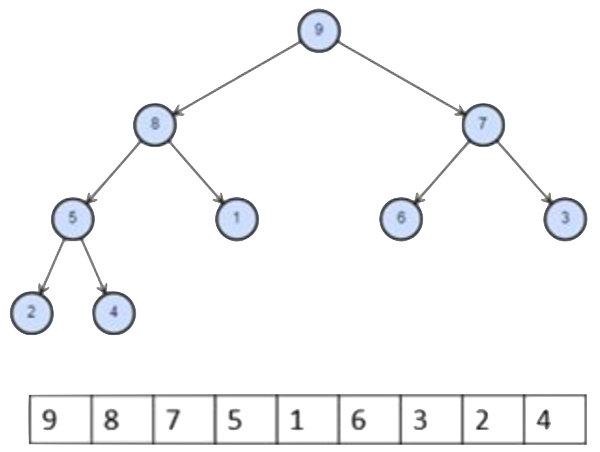
\includegraphics[width=.2\textwidth]{input/06-Graph-fig/heapSort}}
%
%Fuente: \textit{Problem Solving in Data Structures  Algorithms Using Python Programming Interview Guide by Hemant Jain}
%
%

